% ============================================================
%  ParamNet -- advisor presentation
%  Compile with pdfLaTeX (Overleaf: Menu > Compiler > pdfLaTeX).
%  Single file, no external images required.
%  Numbers follow the 23 July 2026 revision of the report
%  (fixed-sigma persistence imager; Matern results pending re-run).
% ============================================================
\documentclass[aspectratio=169,10pt]{beamer}

\usepackage[T1]{fontenc}
\IfFileExists{lmodern.sty}{\usepackage{lmodern}}{}
\usepackage{amsmath,amssymb}
\usepackage{ifthen}
\usepackage{adjustbox}
\usepackage{tikz}
\usepackage{pgfplots}
\pgfplotsset{compat=1.18}
\usetikzlibrary{positioning,arrows.meta,fit,backgrounds,calc,decorations.pathreplacing}

% ---------- look & feel -------------------------------------
\usetheme{default}
\usecolortheme{default}
\setbeamertemplate{navigation symbols}{}
\setbeamerfont{frametitle}{size=\large,series=\bfseries}
\setbeamercolor{frametitle}{fg=black}
\setbeamertemplate{frametitle}{\vspace{0.30cm}\insertframetitle\vspace{-0.15cm}}
\setbeamertemplate{footline}{\hfill\scriptsize\color{gray}\insertframenumber\hspace{0.4cm}\vspace{0.15cm}}

% ---------- palette (matches the hand drawings) --------------
\definecolor{cblue}{HTML}{2E9FD6}   % CONV
\definecolor{cgreen}{HTML}{16A085}  % POOL / DROP
\definecolor{cpurple}{HTML}{A400C0} % LINEAR / DENSE
\definecolor{corange}{HTML}{E8622A} % LayerNorm
\definecolor{cred}{HTML}{E8192C}    % annotations / tensor shapes
\definecolor{cgray}{HTML}{555555}
\definecolor{cgood}{HTML}{16A085}
\definecolor{cbad}{HTML}{E8622A}

% one clean rectangle per legend entry (plots with error bars
% otherwise draw the swatch twice)
\pgfplotsset{
  barlegend/.style={
    legend image code/.code={\draw[#1] (0cm,-0.075cm) rectangle (0.3cm,0.075cm);}},
}

% ---------- block styles -------------------------------------
\tikzset{
  blk/.style   ={draw=none,text=white,font=\ttfamily\scriptsize,
                 minimum width=1.9cm,minimum height=0.42cm,inner sep=1pt},
  conv/.style  ={blk,fill=cblue},
  pool/.style  ={blk,fill=cgreen},
  lin/.style   ={blk,fill=cpurple},
  norm/.style  ={blk,fill=corange},
  tens/.style  ={font=\scriptsize,text=cred},
  note/.style  ={font=\scriptsize,text=cgray},
  arr/.style   ={-{Latex[length=2mm]},thick,cgray},
  box/.style   ={draw=cgray,thick,rounded corners=1pt,inner sep=2pt},
}

% every diagram is shrunk to fit the frame if it would overflow
\newenvironment{fitpic}
  {\begin{adjustbox}{max width=\textwidth,max totalheight=0.74\textheight,center}\begin{tikzpicture}}
  {\end{tikzpicture}\end{adjustbox}}

% ---------- reusable pictures --------------------------------
\newcommand{\pointcloud}[1]{%
\begin{scope}[shift={#1}]
 \foreach \x/\y in {0.20/1.05,0.32/1.22,0.15/0.90,0.38/0.98,0.26/0.78,
                    0.55/1.30,0.62/1.12,0.48/1.42,
                    0.95/0.62,1.08/0.75,0.88/0.48,1.15/0.55,1.02/0.38,0.80/0.68,
                    1.45/1.05,1.58/1.18,1.38/0.90,1.62/0.95,1.50/1.28,
                    1.72/0.35,1.85/0.48,1.95/0.28,1.78/0.18,2.02/0.45}
   {\fill[black] (\x,\y) circle (0.035);}
\end{scope}}

\newcommand{\pdplot}[1]{%
\begin{scope}[shift={#1}]
 \draw[cgray,thick,-{Latex[length=1.2mm]}] (0,0) -- (1.05,0);
 \draw[cgray,thick,-{Latex[length=1.2mm]}] (0,0) -- (0,0.95);
 \draw[dashed,cgray] (0,0) -- (0.85,0.85);
 \foreach \x/\y in {0.15/0.42,0.25/0.62,0.34/0.55,0.45/0.80,0.20/0.30,0.52/0.72}
   {\fill[cblue] (\x,\y) circle (0.028);}
 \foreach \x/\y in {0.30/0.36,0.42/0.50,0.55/0.62,0.62/0.70,0.18/0.24}
   {\fill[cred] (\x,\y) circle (0.028);}
\end{scope}}

\newcommand{\pigrid}[2]{%
\begin{scope}[shift={#1}]
 \fill[cred!75] (0.2,0.4) rectangle (0.6,0.8);
 \fill[cred!45] (0.4,0.2) rectangle (0.6,0.4);
 \fill[cred!45] (0.2,0.8) rectangle (0.4,1.0);
 \draw[step=0.2,gray!60,very thin] (0,0) grid (1.0,1.0);
 \draw[black,thick] (0,0) rectangle (1.0,1.0);
 \node[above,font=\tiny\ttfamily,inner sep=1pt] at (0.5,1.0) {#2};
\end{scope}}

% CoordConv PI encoder stack: #1 = node prefix, #2 = coordinate of top block
\newcommand{\encoderstack}[2]{%
 \node[conv] (#1a) at #2 {CONV2D};
 \node[pool,below=0pt of #1a] (#1b) {POOL};
 \node[conv,below=0pt of #1b] (#1c) {CONV2D};
 \node[pool,below=0pt of #1c] (#1d) {POOL};
 \node[conv,below=0pt of #1d] (#1e) {CONV2D};
 \node[pool,below=0pt of #1e] (#1f) {POOL};
 \node[lin,below=0pt of #1f]  (#1g) {LINEAR};
 \node[box,fit=(#1a)(#1g)] (#1box) {};}

% compact unlabelled encoder (towers slide)
\newcommand{\minienc}[2]{%
 \node[conv,minimum width=1.4cm,minimum height=0.26cm] (#1a) at #2 {};
 \node[pool,minimum width=1.4cm,minimum height=0.26cm,below=0pt of #1a] (#1b) {};
 \node[conv,minimum width=1.4cm,minimum height=0.26cm,below=0pt of #1b] (#1c) {};
 \node[pool,minimum width=1.4cm,minimum height=0.26cm,below=0pt of #1c] (#1d) {};
 \node[conv,minimum width=1.4cm,minimum height=0.26cm,below=0pt of #1d] (#1e) {};
 \node[pool,minimum width=1.4cm,minimum height=0.26cm,below=0pt of #1e] (#1f) {};
 \node[lin,minimum width=1.4cm,minimum height=0.26cm,below=0pt of #1f] (#1g) {};
 \node[box,fit=(#1a)(#1g)] (#1box) {};}

% MLP regression head
\newcommand{\headstack}[2]{%
 \node[lin]  (#1a) at #2 {LINEAR};
 \node[pool,below=0pt of #1a] (#1b) {DROP};
 \node[lin,below=0pt of #1b]  (#1c) {LINEAR};
 \node[pool,below=0pt of #1c] (#1d) {DROP};
 \node[lin,below=0pt of #1d]  (#1e) {LINEAR};
 \node[box,fit=(#1a)(#1e)] (#1box) {};}

% Conv1d fusion over the scale axis; #3 = pool | flatten
\newcommand{\fusionstack}[3]{%
 \node[conv] (#1a) at #2 {CONV1D};
 \node[norm,below=0pt of #1a] (#1b) {LN+ReLU};
 \node[conv,below=0pt of #1b] (#1c) {CONV1D};
 \node[norm,below=0pt of #1c] (#1d) {LN+ReLU};
 \ifthenelse{\equal{#3}{pool}}
   {\node[pool,below=0pt of #1d] (#1e) {POOL};}
   {\node[blk,fill=cgray!45,text=cgray,below=0pt of #1d] (#1e) {FLATTEN};}
 \node[box,fit=(#1a)(#1e)] (#1box) {};}

% ---------- section title pages ------------------------------
\AtBeginSection[]{%
\begin{frame}[plain]
 \centering\vfill
 {\usebeamerfont{title}\Large\bfseries\insertsectionhead}\\[0.35cm]
 {\color{cred}\rule{4cm}{1.2pt}}
 \vfill
\end{frame}}

% ============================================================
\title{\bfseries ParamNet}
\subtitle{Estimating point-process parameters from topological features\\[2pt]
\small nested Thomas}
\author{Flavio Gualtieri}
\date{July 2026}

\begin{document}

\begin{frame}[plain]
 \titlepage
\end{frame}

% ============================================================
\begin{frame}{The task}
\vspace{0.3cm}
\begin{fitpic}
 \pointcloud{(0,0)}
 \draw[cgray,thick] (-0.15,-0.15) rectangle (2.25,1.65);
 \node[note,align=center] at (1.05,-0.6)
     {point cloud from a\\ stochastic point process};

 \draw[arr] (2.7,0.75) -- (5.3,0.75);
 \node[note,anchor=south] at (4.0,0.85) {FEATURIZE + NN};

 \node[tens,anchor=west] at (5.6,0.75) {PARAMETERS};
\end{fitpic}

\vfill

\begin{minipage}{0.92\textwidth}
{\color{cgray}\scriptsize
\textbf{Notes}
\begin{itemize}
 \setlength{\itemsep}{0.1em}
 \item Nested Thomas parameters: parent intensity $\kappa$,
       mean offspring counts $\mu_1,\mu_2$, and dispersal scales
       $\sigma_1,\sigma_2$.
 \item Training objective: MSE in standardized log-$z$ target space.
\end{itemize}
}
\end{minipage}
\end{frame}

% ============================================================

\begin{frame}{\texttt{vihrs} --- Vihrs (2022), re-implemented}
\begin{fitpic}

% --- cloud with radius r
 \begin{scope}[shift={(0,2.5)},scale=0.8]
  \pointcloud{(0,0)}
  \draw[cred,thick] (1.0,0.55) circle (0.55);
  \fill[cred] (1.0,0.55) circle (0.05);
  \draw[cred,thick,-{Latex[length=1.2mm]}] (1.0,0.55) -- (1.55,0.55);
  \node[tens,anchor=south] at (1.3,0.60) {$r$};
 \end{scope}

 \draw[arr] (2.2,3.1) -- (2.9,3.1);

% --- L(r)-r curve
 \begin{scope}[shift={(3.1,2.5)}]
  \draw[cgray,thick,-{Latex[length=1.2mm]}] (0,0) -- (1.3,0);
  \draw[cgray,thick,-{Latex[length=1.2mm]}] (0,0) -- (0,1.15);
  \draw[cred,very thick] plot[smooth,tension=0.8]
    coordinates {(0.05,0.05) (0.3,0.45) (0.6,0.72) (0.9,0.82) (1.2,0.86)};
  \node[note,anchor=north] at (0.7,-0.02) {$r$};
  \node[tens,anchor=west] at (0.1,1.05) {$L(r)-r$};
 \end{scope}

 \draw[arr] (4.6,3.1) -- (5.3,3.1);
 \node[tens,anchor=west] at (5.4,3.25)
  {$\big[\,L(r_1)-r_1,\ \dots,\ L(r_m)-r_m\,\big]$};
 \node[note,anchor=west] at (5.4,2.75) {513 points, \ $r_{\max}=0.25$};

% --- 1D CNN chain
 \draw[arr] (7.4,2.5) -- (7.4,1.8);
 \node[note,anchor=west] at (7.5,2.15) {normalize};

 \node[conv,minimum width=1.5cm] (v1) at (1.75,1.4) {CONV1D};
 \node[pool,minimum width=1.5cm,right=0.1cm of v1] (v2) {POOL};
 \node[conv,minimum width=1.5cm,right=0.1cm of v2] (v3) {CONV1D};
 \node[pool,minimum width=1.5cm,right=0.1cm of v3] (v4) {POOL};
 \node[conv,minimum width=1.5cm,right=0.1cm of v4] (v5) {CONV1D};
 \node[box,fit=(v1)(v5)] (vbox) {};
 \node[note,anchor=east] at (0.85,1.4) {1D CNN};

 \draw[arr] (vbox.east) -- (9.6,1.4);

 \node[lin,minimum width=2.1cm,minimum height=0.8cm,align=center] (dense) at (10.8,1.4)
   {DENSE\\$64 \to 32$};
 \node[tens] (logn) at (10.8,2.6) {$\log N$};
 \draw[arr] (logn.south) -- (dense.north);

 \node[tens] (params) at (10.8,0.25) {PARAMS};
 \draw[arr] (dense.south) -- (params.north);
\end{fitpic}

\vfill

\begin{minipage}{0.92\textwidth}
{\color{cgray}\scriptsize
\textbf{Notes}
\begin{itemize}
 \setlength{\itemsep}{0.1em}
 \item No TDA features at all
\end{itemize}
}
\end{minipage}

\end{frame}

% ============================================================

\begin{frame}{From point cloud to persistence images}
\begin{fitpic}

 \pointcloud{(0,0.8)}
 \draw[cgray,thick] (-0.15,0.65) rectangle (2.25,2.45);

 \draw[arr] (2.4,1.6) -- (2.9,2.55);
 \draw[arr] (2.4,1.6) -- (2.9,0.65);

 \node[tens] (d1) at (3.55,2.6) {DTM($m_1$)};
 \node[note] at (3.55,1.6) {$\vdots$};
 \node[tens] (dk) at (3.55,0.6) {DTM($m_K$)};

 \draw[arr] (d1.east) -- ++(0.5,0);
 \draw[arr] (dk.east) -- ++(0.5,0);

 \pdplot{(4.75,2.1)}
 \pdplot{(4.75,0.1)}
 \node[note] at (5.3,1.6) {$\vdots$};

 \draw[arr] (5.95,2.6) -- (6.35,2.6);
 \draw[arr] (5.95,0.6) -- (6.35,0.6);

 \pigrid{(6.5,2.1)}{H0}
 \pigrid{(7.7,2.1)}{H1}
 \pigrid{(6.5,0.1)}{H0}
 \pigrid{(7.7,0.1)}{H1}
 \node[note] at (7.0,1.6) {$\vdots$};
 \node[note] at (8.2,1.6) {$\vdots$};

 \draw[arr] (8.9,1.6) -- (9.5,1.6);
 \node[tens,anchor=west] at (9.6,1.75) {$(B,\,K,\,2,\,64,\,64)$};

\end{fitpic}

\vfill

\begin{minipage}{0.92\textwidth}
{\color{cgray}\scriptsize
\textbf{Notes}
\begin{itemize}
 \setlength{\itemsep}{0.1em}
 \item DTM scale based on mass fraction $m$, \ \ $k=\mathrm{round}(m\cdot N)$ recomputed per cloud
 \item swept grid: $m\in\{0.01,\,0.02,\,0.04,\,0.10,\,0.20,\,0.45,\,0.90\}$
 \item $64\times 64$ raster, fixed $\sigma = 2$ px, exact per-pixel integration
\end{itemize}
}
\end{minipage}
\end{frame}

% ------------------------------------------------------------
\begin{frame}{Shared building block: the CoordConv PI encoder}
\begin{fitpic}

 \pigrid{(0,1.0)}{H0}
 \pigrid{(1.2,1.0)}{H1}
 \node[tens,anchor=north] at (1.1,0.85) {$(2,\,64,\,64)$};
 \node[note,anchor=north] at (1.1,0.40) {one DTM scale};

 \draw[arr] (2.5,1.5) -- (3.6,1.5);
 \node[note,align=center,anchor=south] at (3.05,1.6) {$+2$ coord\\ channels};

 \encoderstack{e}{(5.0,2.9)}

 \node[note,anchor=west] at (6.2, 2.9) {$4 \to 32 \to 64 \to 128$};
 \node[note,anchor=west] at (6.2,0.30) {$128 \to 64$};

 \draw[arr] (5.0,-0.20) -- (5.0,-0.75);
 \node[tens,anchor=north] at (5.0,-0.85) {$64$-dim embedding};
\end{fitpic}

\vfill

\begin{minipage}{0.92\textwidth}
{\color{cgray}\scriptsize
\textbf{Notes}
\begin{itemize}
 \setlength{\itemsep}{0.1em}
 \item Dropout2d between blocks
 \item Global average pooling
 \item Every model variant below differs \emph{only} in how the $K$ embeddings are fused
\end{itemize}
}
\end{minipage}
\end{frame}

% ============================================================

% ---------------- 1. flat concat ----------------------------
\begin{frame}{\texttt{pi\_multik} --- flat concatenation (late fusion)}
\begin{fitpic}
 \node[tens] (in) at (0.7,1.5) {$(K,\,2,\,64,\,64)$};
 \draw[arr] (1.8,1.5) -- (2.5,1.5);

 \encoderstack{e}{(3.5,2.9)}
 \node[note,anchor=south] at (3.5,3.25) {SHARED ENCODER};

 \draw[arr] (4.6,1.5) -- (5.3,1.5);
 \node[tens] (emb) at (6.1,1.5) {$(K,\,64)$};
 \draw[arr] (6.9,1.5) -- (7.6,1.5);
 \node[tens,align=center] (flat) at (8.7,1.5) {$(K\!\cdot\!64,\,)$};
 \node[note,anchor=south,align=center] at (8.7,1.85) {CONCAT\\ (order-blind)};

 \draw[arr] (9.8,1.5) -- (10.5,1.5);
 \headstack{h}{(11.5,2.4)}
 \node[note,anchor=south] at (11.5,2.75) {HEAD};
 \draw[arr] (11.5,0.2) -- (11.5,-0.35);
 \node[tens,anchor=north] at (11.5,-0.45) {PARAMS};
\end{fitpic}

\vfill

\begin{minipage}{0.92\textwidth}
{\color{cgray}\scriptsize
\textbf{Notes}
\begin{itemize}
 \setlength{\itemsep}{0.1em}
 \item No notion of scale adjacency --- the $K$ embeddings are just stacked
\end{itemize}
}
\end{minipage}

\end{frame}

% ---------------- 3. scaleconv ------------------------------
\begin{frame}{\texttt{pi\_multik\_scaleconv} --- 1D convolution along the scale axis}
\begin{fitpic}
 \node[tens] (in) at (0.7,1.5) {$(K,\,2,\,64,\,64)$};
 \draw[arr] (1.8,1.5) -- (2.5,1.5);

 \encoderstack{e}{(3.5,2.9)}
 \node[note,anchor=south] at (3.5,3.25) {SHARED ENCODER};

 \draw[arr] (4.6,1.5) -- (5.2,1.5);
 \node[tens] (emb) at (5.9,1.5) {$(K,\,64)$};
 \node[note,anchor=south,align=center] at (5.9,1.85) {ORDERED\\ SEQUENCE};
 \draw[arr] (6.6,1.5) -- (7.2,1.5);

 \fusionstack{f}{(8.3,2.55)}{pool}
 \node[note,anchor=south] at (8.3,2.90) {ScaleConvFusion};

 \draw[arr] (9.4,1.5) -- (10.0,1.5);
 \node[tens] (fused) at (10.7,1.5) {$(128,\,)$};
 \draw[arr] (11.4,1.5) -- (12.0,1.5);

 \headstack{h}{(13.0,2.4)}
 \node[note,anchor=south] at (13.0,2.75) {HEAD};
 \draw[arr] (13.0,0.2) -- (13.0,-0.35);
 \node[tens,anchor=north] at (13.0,-0.45) {PARAMS};
\end{fitpic}

\vfill

\begin{minipage}{0.92\textwidth}
{\color{cgray}\scriptsize
\textbf{Notes}
\begin{itemize}
 \setlength{\itemsep}{0.1em}
 \item Mixes adjacent scales, then pools the scale axis away $\Rightarrow$ \ head input $=129$ for \emph{any} $K$
 \item Only variant whose head width does not grow with the number of scales
\end{itemize}
}
\end{minipage}

\end{frame}

% ---------------- 4. towers ---------------------------------
\begin{frame}{\texttt{pi\_multik\_towers} --- independent per-scale encoders}
\begin{fitpic}

 \node[tens] (i1) at (0.4,3.0) {$m_1$};
 \node[note] at (0.4,2.0) {$\vdots$};
 \node[tens] (ik) at (0.4,1.0) {$m_K$};

 \draw[arr] (0.9,3.0) -- (1.5,3.0);
 \draw[arr] (0.9,1.0) -- (1.5,1.0);

 \minienc{t}{(2.5,3.85)}
 \minienc{u}{(2.5,1.85)}
 \node[note] at (2.5,2.0) {$\vdots$};

 \draw[arr] (3.3,3.0) -- (3.9,3.0);
 \draw[arr] (3.3,1.0) -- (3.9,1.0);
 \node[tens,anchor=west] at (4.0,3.0) {$(64,)$};
 \node[tens,anchor=west] at (4.0,1.0) {$(64,)$};

 \draw[decorate,decoration={brace,amplitude=5pt},cgray] (5.1,3.35) -- (5.1,0.65);
 \node[tens,anchor=west] at (5.5,2.0) {$(K,\,64)$};

 \draw[arr] (6.5,2.0) -- (7.1,2.0);
 \fusionstack{f}{(8.2,3.05)}{flatten}
 \node[note,anchor=south] at (8.2,3.40) {TowerConv (no pooling)};

 \draw[arr] (9.3,2.0) -- (9.9,2.0);
 \node[tens] (fused) at (10.7,2.0) {$(128K,\,)$};
 \draw[arr] (11.5,2.0) -- (12.1,2.0);

 \headstack{h}{(13.1,2.9)}
 \node[note,anchor=south] at (13.1,3.25) {HEAD};
 \draw[arr] (13.1,0.7) -- (13.1,0.15);
 \node[tens,anchor=north] at (13.1,0.05) {PARAMS};
\end{fitpic}

\vfill

\begin{minipage}{0.92\textwidth}
{\color{cgray}\scriptsize
\textbf{Notes}
\begin{itemize}
 \setlength{\itemsep}{0.1em}
 \item Most parameters of all the variants
 \item Same Conv1d recipe as \texttt{scaleconv}, but flattened instead of pooled
\end{itemize}
}
\end{minipage}
\end{frame}

% ---------------- summary of the four -----------------------
\begin{frame}{Four ways to fuse $K$ scales}
\centering
\vspace{0.2cm}
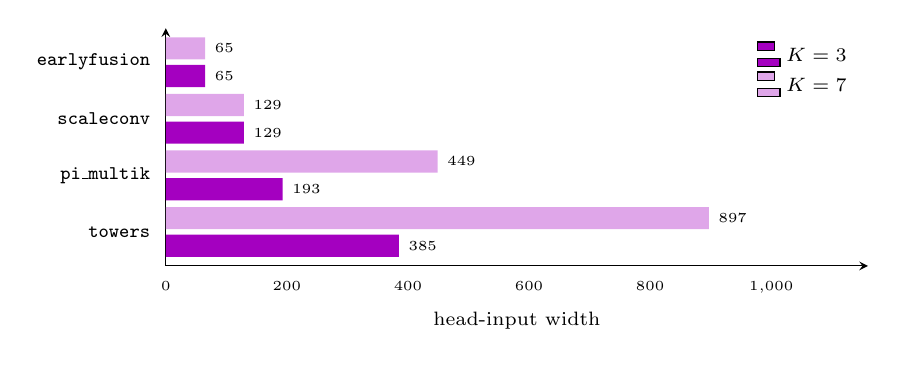
\begin{tikzpicture}
\begin{axis}[barlegend,
  xbar, width=10.5cm, height=4.6cm,
  bar width=8pt,
  xmin=0, xmax=1160,
  xlabel={\scriptsize head-input width},
  ytick={0,1,2,3},
  yticklabels={{\ttfamily towers},{\ttfamily pi\_multik},{\ttfamily scaleconv},{\ttfamily earlyfusion}},
  yticklabel style={font=\scriptsize},
  xticklabel style={font=\tiny},
  ymin=-0.6, ymax=3.6, enlarge y limits=false,
  nodes near coords, nodes near coords style={font=\tiny},
  axis lines=left, tick style={draw=none},
  legend style={draw=none,fill=none,font=\scriptsize,at={(0.99,0.97)},anchor=north east},
]
\addplot[fill=cpurple,draw=none,bar shift=-5pt] coordinates {(385,0) (193,1) (129,2) (65,3)};
\addplot[fill=cpurple!35,draw=none,bar shift=5pt] coordinates {(897,0) (449,1) (129,2) (65,3)};
\legend{$K=3$,$K=7$}
\end{axis}
\end{tikzpicture}

\vfill

\begin{minipage}{0.92\textwidth}
{\color{cgray}\scriptsize
\textbf{Notes}
\begin{itemize}
 \setlength{\itemsep}{0.1em}
 \item Only \texttt{scaleconv} and \texttt{earlyfusion} keep a fixed head width as scales are added
\end{itemize}
}
\end{minipage}

\end{frame}

% ============================================================

\begin{frame}{One DTM scale at a time --- finer is better}
\centering
\vspace{0.1cm}
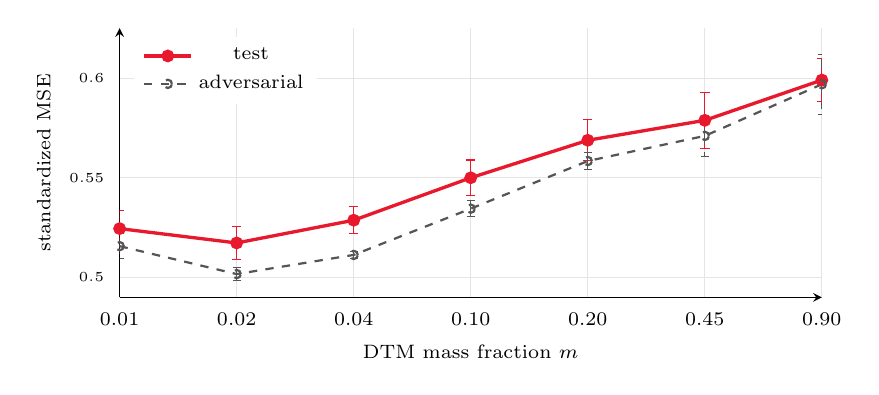
\begin{tikzpicture}
\begin{axis}[
  width=10.5cm, height=5.0cm,
  xtick={1,2,3,4,5,6,7},
  xticklabels={0.01,0.02,0.04,0.10,0.20,0.45,0.90},
  xlabel={\scriptsize DTM mass fraction $m$},
  ylabel={\scriptsize standardized MSE},
  xticklabel style={font=\scriptsize}, yticklabel style={font=\tiny},
  ymin=0.49, ymax=0.625,
  axis lines=left, tick style={draw=none},
  grid=major, grid style={gray!20},
  legend style={draw=none,font=\scriptsize,at={(0.02,0.97)},anchor=north west},
]
\addplot[cred,very thick,mark=*,mark size=1.7pt,
  error bars/.cd, y dir=both, y explicit]
 coordinates {(1,0.5245) +- (0,0.0091)
              (2,0.5173) +- (0,0.0083)
              (3,0.5287) +- (0,0.0067)
              (4,0.5500) +- (0,0.0089)
              (5,0.5688) +- (0,0.0103)
              (6,0.5788) +- (0,0.0141)
              (7,0.5990) +- (0,0.0108)};
\addplot[cgray,thick,dashed,mark=o,mark size=1.5pt,
  error bars/.cd, y dir=both, y explicit]
 coordinates {(1,0.5157) +- (0,0.0063)
              (2,0.5017) +- (0,0.0033)
              (3,0.5113) +- (0,0.0018)
              (4,0.5345) +- (0,0.0039)
              (5,0.5584) +- (0,0.0044)
              (6,0.5710) +- (0,0.0102)
              (7,0.5969) +- (0,0.0151)};
\legend{test,adversarial}
\end{axis}
\end{tikzpicture}

\vfill

\begin{minipage}{0.92\textwidth}
{\color{cgray}\scriptsize
\textbf{Notes}
\begin{itemize}
 \setlength{\itemsep}{0.1em}
 \item $n=3$ seeds
 \item Architecture fixed, only the input scale changes
 \item Best single scale: $m=0.02$
\end{itemize}
}
\end{minipage}

\end{frame}

% ------------------------------------------------------------
\begin{frame}{Multi-scale: the fine scales carry the signal}
\centering
\vspace{0.1cm}
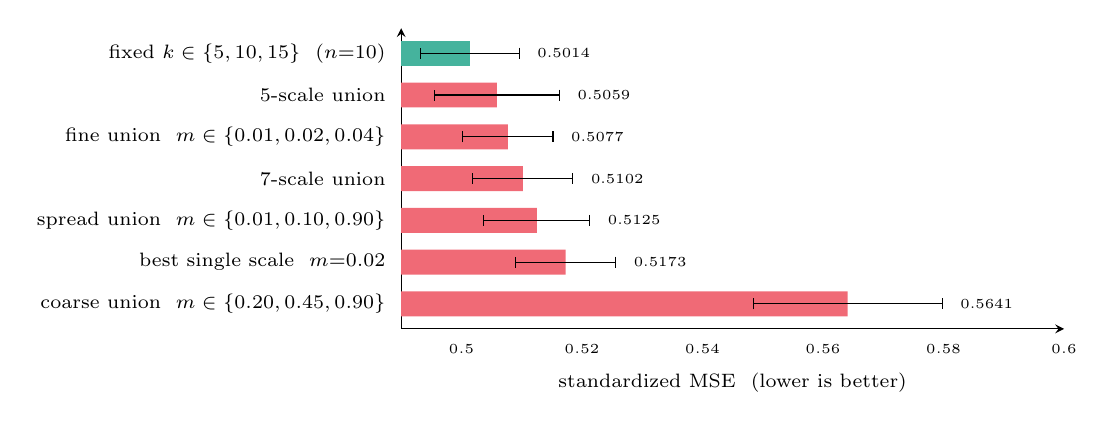
\begin{tikzpicture}
\begin{axis}[
  xbar, width=10.0cm, height=5.4cm, bar width=9pt,
  xmin=0.49, xmax=0.60,
  ytick={0,1,2,3,4,5,6},
  yticklabels={{coarse union \ $m\in\{0.20,0.45,0.90\}$},
               {best single scale \ $m{=}0.02$},
               {spread union \ $m\in\{0.01,0.10,0.90\}$},
               {7-scale union},
               {fine union \ $m\in\{0.01,0.02,0.04\}$},
               {5-scale union},
               {fixed $k\in\{5,10,15\}$ \ ($n{=}10$)}},
  yticklabel style={font=\scriptsize}, xticklabel style={font=\tiny},
  xlabel={\scriptsize standardized MSE \ (lower is better)},
  ymin=-0.6, ymax=6.6, enlarge y limits=false,
  axis lines=left, tick style={draw=none},
]
\addplot[fill=cred!65,draw=none,bar shift=0pt,
  error bars/.cd, x dir=both, x explicit]
 coordinates {(0.5641,0) +- (0.0157,0)
              (0.5173,1) +- (0.0083,0)
              (0.5125,2) +- (0.0088,0)
              (0.5102,3) +- (0.0083,0)
              (0.5077,4) +- (0.0075,0)
              (0.5059,5) +- (0.0104,0)};
\addplot[fill=cgood!80,draw=none,bar shift=0pt,
  error bars/.cd, x dir=both, x explicit]
 coordinates {(0.5014,6) +- (0.0082,0)};
% value labels, placed clear of the error-bar caps
\node[font=\tiny,anchor=west,xshift=3pt] at (axis cs:0.5798,0) {0.5641};
\node[font=\tiny,anchor=west,xshift=3pt] at (axis cs:0.5256,1) {0.5173};
\node[font=\tiny,anchor=west,xshift=3pt] at (axis cs:0.5213,2) {0.5125};
\node[font=\tiny,anchor=west,xshift=3pt] at (axis cs:0.5185,3) {0.5102};
\node[font=\tiny,anchor=west,xshift=3pt] at (axis cs:0.5152,4) {0.5077};
\node[font=\tiny,anchor=west,xshift=3pt] at (axis cs:0.5163,5) {0.5059};
\node[font=\tiny,anchor=west,xshift=3pt] at (axis cs:0.5096,6) {0.5014};
\end{axis}
\end{tikzpicture}

\vfill

\begin{minipage}{0.92\textwidth}
{\color{cgray}\scriptsize
\textbf{Notes}
\begin{itemize}
 \setlength{\itemsep}{0.1em}
 \item Every union containing a fine scale lands in $0.506$--$0.513$
 \item The coarse-only union is clearly worse
 \item Fixed $k$ is best overall
\end{itemize}
}
\end{minipage}

\end{frame}

% ============================================================
\begin{frame}{Every TDA variant beats \texttt{vihrs}}
\centering
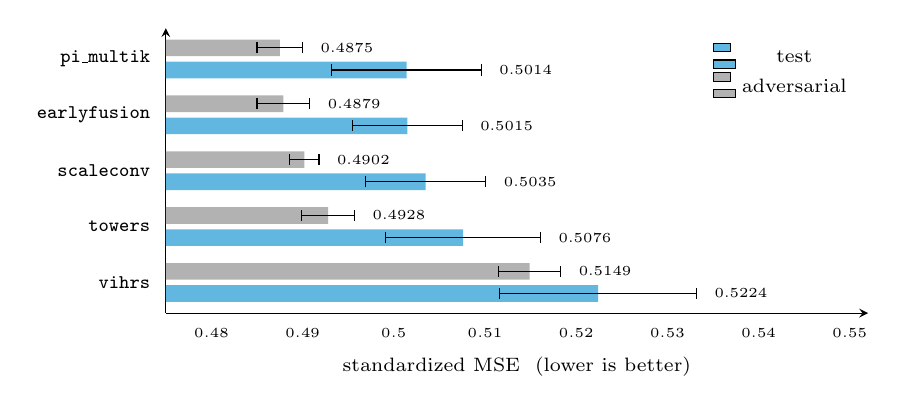
\begin{tikzpicture}
\begin{axis}[area legend,
  xbar, width=10.5cm, height=5.2cm, bar width=6pt,
  xmin=0.475, xmax=0.552,
  ytick={0,1,2,3,4},
  yticklabels={{\ttfamily vihrs},{\ttfamily towers},{\ttfamily scaleconv},{\ttfamily earlyfusion},{\ttfamily pi\_multik}},
  yticklabel style={font=\scriptsize}, xticklabel style={font=\tiny},
  xlabel={\scriptsize standardized MSE \ (lower is better)},
  ymin=-0.55, ymax=4.55, enlarge y limits=false,
  axis lines=left, tick style={draw=none},
  legend style={draw=none,fill=none,font=\scriptsize,at={(0.99,0.97)},anchor=north east},
]
\addplot[fill=cblue!75,draw=none,bar shift=-4pt,
  error bars/.cd, x dir=both, x explicit]
 coordinates {(0.5224,0) +- (0.0108,0)
              (0.5076,1) +- (0.0085,0)
              (0.5035,2) +- (0.0066,0)
              (0.5015,3) +- (0.0060,0)
              (0.5014,4) +- (0.0082,0)};
\addplot[fill=cgray!45,draw=none,bar shift=4pt,
  error bars/.cd, x dir=both, x explicit]
 coordinates {(0.5149,0) +- (0.0034,0)
              (0.4928,1) +- (0.0029,0)
              (0.4902,2) +- (0.0016,0)
              (0.4879,3) +- (0.0029,0)
              (0.4875,4) +- (0.0025,0)};
\legend{test,adversarial}
% test labels (lower bar of each pair)
\node[font=\tiny,anchor=west,xshift=3pt,yshift=-4pt] at (axis cs:0.5332,0) {0.5224};
\node[font=\tiny,anchor=west,xshift=3pt,yshift=-4pt] at (axis cs:0.5161,1) {0.5076};
\node[font=\tiny,anchor=west,xshift=3pt,yshift=-4pt] at (axis cs:0.5101,2) {0.5035};
\node[font=\tiny,anchor=west,xshift=3pt,yshift=-4pt] at (axis cs:0.5075,3) {0.5015};
\node[font=\tiny,anchor=west,xshift=3pt,yshift=-4pt] at (axis cs:0.5096,4) {0.5014};
% adversarial labels (upper bar of each pair)
\node[font=\tiny,anchor=west,xshift=3pt,yshift=4pt] at (axis cs:0.5183,0) {0.5149};
\node[font=\tiny,anchor=west,xshift=3pt,yshift=4pt] at (axis cs:0.4957,1) {0.4928};
\node[font=\tiny,anchor=west,xshift=3pt,yshift=4pt] at (axis cs:0.4918,2) {0.4902};
\node[font=\tiny,anchor=west,xshift=3pt,yshift=4pt] at (axis cs:0.4908,3) {0.4879};
\node[font=\tiny,anchor=west,xshift=3pt,yshift=4pt] at (axis cs:0.4900,4) {0.4875};
\end{axis}
\end{tikzpicture}

\vfill

\begin{minipage}{0.92\textwidth}
{\color{cgray}\scriptsize
\textbf{Notes}
\begin{itemize}
 \setlength{\itemsep}{0.1em}
 \item $n=10$ on both sides, $k\in\{5,10,15\}$
 \item Gap $\approx0.021$
 \item Flat concat and early fusion tied for best --- fancier fusions don't help
\end{itemize}
}
\end{minipage}

\end{frame}

% ------------------------------------------------------------
\begin{frame}{Where the advantage lives (per target)}
\centering
\vspace{0.1cm}
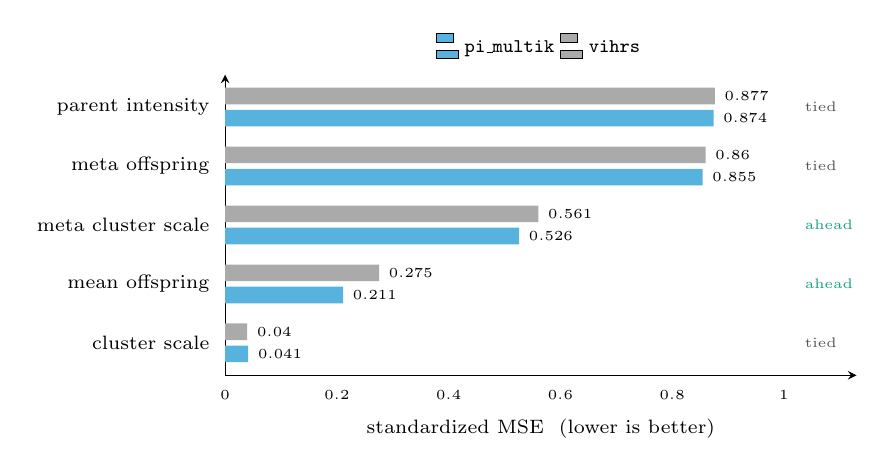
\begin{tikzpicture}
\begin{axis}[area legend,
  xbar, width=9.6cm, height=5.4cm, bar width=6pt,
  xmin=0, xmax=1.13,
  ytick={0,1,2,3,4},
  yticklabels={{cluster scale},{mean offspring},{meta cluster scale},{meta offspring},{parent intensity}},
  yticklabel style={font=\scriptsize}, xticklabel style={font=\tiny},
  xtick={0,0.2,0.4,0.6,0.8,1.0},
  xlabel={\scriptsize standardized MSE \ (lower is better)},
  ymin=-0.55, ymax=4.55, enlarge y limits=false,
  axis lines=left, tick style={draw=none},
  legend style={draw=none,fill=none,font=\scriptsize,at={(0.5,1.02)},anchor=south,legend columns=2},
  nodes near coords, nodes near coords style={font=\tiny},
  every node near coord/.append style={/pgf/number format/.cd,fixed,precision=3},
]
\addplot[fill=cblue!80,draw=none,bar shift=-4pt]
  coordinates {(0.0413,0) (0.2109,1) (0.5261,2) (0.8546,3) (0.8740,4)};
\addplot[fill=cgray!50,draw=none,bar shift=4pt]
  coordinates {(0.0395,0) (0.2754,1) (0.5607,2) (0.8600,3) (0.8765,4)};
\legend{\texttt{pi\_multik},\texttt{vihrs}}

\node[font=\tiny,text=cgood,anchor=west] at (axis cs:1.02,1) {ahead};
\node[font=\tiny,text=cgood,anchor=west] at (axis cs:1.02,2) {ahead};
\node[font=\tiny,text=cgray,anchor=west]  at (axis cs:1.02,0) {tied};
\node[font=\tiny,text=cgray,anchor=west]  at (axis cs:1.02,3) {tied};
\node[font=\tiny,text=cgray,anchor=west]  at (axis cs:1.02,4) {tied};
\end{axis}
\end{tikzpicture}

\vfill

\begin{minipage}{0.92\textwidth}
{\color{cgray}\scriptsize
\textbf{Notes}
\begin{itemize}
 \setlength{\itemsep}{0.1em}
 \item The advantage is \texttt{meta cluster scale} and \texttt{mean offspring} only
 \item Both coarse targets look capped for \emph{either} feature set
\end{itemize}
}
\end{minipage}

\end{frame}

\end{document}